% EDGE paper. Build: pdflatex -> bibtex -> pdflatex -> pdflatex.
\PassOptionsToPackage{table}{xcolor}
\documentclass[pdflatex,sn-mathphys-ay]{sn-jnl}

\usepackage{graphicx}
\usepackage{amsmath,amssymb,amsfonts}
\usepackage{booktabs}
\usepackage{multirow}
\usepackage{array}
\usepackage{adjustbox}
\usepackage[table]{xcolor}
\usepackage[title]{appendix}
\graphicspath{{figures/}}
\makeatletter
\def\input@path{{tables/}{sections/}}
\makeatother

\theoremstyle{thmstyleone}
\newtheorem{theorem}{Theorem}
\newtheorem{proposition}{Proposition}
\raggedbottom

% --- EDGE notation, identical to the software and the companion papers
\newcommand{\pibar}{\overline{\hat{\pi}}}
\newcommand{\DEFp}[1]{\textsf{EDGE-poly}\ensuremath{_{#1}}}
\newcommand{\DEFsym}{\textsf{EDGE-sym}}
\newcommand{\DEFstk}{\textsf{EDGE-stk}}
\newcommand{\DEFname}{\textsf{EDGE}}
\newcommand{\EFname}{\textsf{HL}$_F$}
\newcommand{\HLname}{\textsf{HL}}
\newcommand{\hd}[2]{\begin{tabular}[b]{@{}c@{}}#1\\#2\end{tabular}}

\begin{document}

\title[A calibration test that tolerates corrupted records]{A grouped calibration test for logistic
regression that tolerates a few corrupted records}

\author*[1]{\fnm{Ebrahim Khaled} \sur{Ebrahim}}\email{ebrahimkhaled@alexu.edu.eg}
\author[1]{\fnm{Osama Abd El-Aziz} \sur{Hussein}}\email{osama.hussein@comm.alexu.edu.eg}
\author[1]{\fnm{Ahmed} \sur{El-Kotory}}\email{ahmed.elkatory@alexu.edu.eg}

\affil[1]{\orgdiv{Department of Applied Statistics, Faculty of Business}, \orgname{Alexandria
University}, \orgaddress{\city{Alexandria}, \postcode{5424074}, \country{Egypt}}}

\abstract{On an otherwise correct model, one record in a thousand with an exaggerated covariate
(multiplied by four) raises the false-alarm rate of Stukel's score test from 5\% to 12\%, and ten
raise it to 63\%. We found no earlier study of how a few corrupted covariate records change the level
of calibration tests for logistic regression. Tests lost their level when they divided a record's
contribution by something the record, or the refit it causes, can make small. Pooling with unit
weights over equal-size risk groups divides a wrong record's residual by its clean groupmates'
variance, which bounds its influence at fixed coefficients. We propose EDGE, which projects grouped
residuals onto a small basis of calibration shapes. For groups formed by predicted risk, its limit
does not depend on the number of groups as it grows with the sample size, making the partition a
setting: fine for power, coarse when records may be wrong. In a prespecified simulation it had power
comparable to Stukel's on clean data and 0.064 more than the ten-group Hosmer--Lemeshow test. With one
and ten exaggerated records per thousand its false-alarm rates were 0.056 and 0.097; at ten groups
they stayed below 0.10 up to about ten exaggerated or five reversed (sign-error) records. In external
validation at ten groups EDGE matched the power of Cox's recalibration test, which lost its level
under corruption. The cumulative-sum test of Sadatsafavi and Petkau was equally protected, while EDGE
was 0.035 more powerful on average, from U-shaped and interaction departures.}

\keywords{Calibration, Goodness-of-fit, Logistic regression, Contaminated data, Hosmer--Lemeshow
test, Clinical prediction model}

\pacs[MSC Classification]{62J12, 62F03, 62P10}

\maketitle

\section{Introduction}\label{sec:intro}

A risk model is calibrated when the risk it reports is the risk the patient carries; a model can rank
patients well and still report the wrong number \citep{vancalster2016hierarchy}. The number is what
decisions use. A model that predicts $8\%$ for patients whose true risk is $5\%$ sends the wrong
patients over a treatment threshold, however well it ranks them. Calibration tests are therefore routine
when prediction models are developed and validated.

This paper makes one point and builds a test on it. A calibration test is fragile to a few corrupted
covariate records when it divides one record's contribution by something that the record, or the
refit it causes, can make small. Pooling residuals over equal-frequency risk groups with unit weights
avoids this, because a wrong record's residual is then divided by the variance of its clean
groupmates. We propose a grouped calibration test, which we call EDGE (Efficient Directed Grouped
Examination). EDGE keeps this protection while avoiding the loss of power that a finer partition
causes in the Hosmer--Lemeshow test. The weights of its asymptotic reference distribution are computed
in closed form from quantities that the model fit has already produced, so it needs no refitting and
no resampling.

For logistic regression with continuous covariates almost every patient has a covariate pattern of
their own, so the Pearson and deviance statistics are sums of cells with one observation each, and
their chi-squared reference fails. One repair standardises the Pearson statistic by its moments
\citep{mccullagh1985,osius1992normal}. The other, by \citet{hosmer1980goodness}, sorts the patients by
predicted risk, cuts them into ten groups and compares observed with expected events in each group.
The Hosmer--Lemeshow test is still the default check of calibration. Its statistic spends one degree
of freedom on each group, so adding groups adds degrees of freedom faster than it adds signal, and the
verdict can change with the number of groups alone \citep{paul2013power}. Its variants repair one
problem at a time. \citet{paul2013power} and \citet{Lai2018} standardise its power in large samples,
\citet{nattino2020assessing} test whether the misfit exceeds a fixed size,
\citet{surjanovic2024generalized} derive a correct reference for a generalized form, and BAGofT
\citep{BAGofT2019} learns the partition on one part of the data and tests on the other.
\citet{hosmer2002goodness} came closest to a directed grouped test, weighting each record's residual
within the groups. None of these variants lets the partition be refined without changing its degrees
of freedom.

Other tests recover power by leaving the grouping behind. \citet{stukel1988generalized} embeds the
logistic link in a two-parameter family and tests the two extra parameters with a score test; it had
the best power against a misspecified link in the comparison of \citet{hosmer1997comparison}. The
GiViTI calibration belt \citep{nattino2014new,nattino2015new}, named after the Italian intensive-care
research group that developed it, fits a polynomial to the calibration curve. The cubic calibration
test adds the square and cube of the fitted linear predictor to a logistic regression of the outcome
on it \citep{pregibon1980goodness,nattino2014new,nattino2015new}. These tests use every record's
residual at its own weight, and that is why they are powerful. It also makes them sensitive to a few
wrong records. Clinical data contain such records: a covariate entered in the wrong units, a misplaced
decimal point, or a count typed as a larger but plausible count, which passes any range check. In this
paper a corrupted covariate is either exaggerated (multiplied by four) or reversed (multiplied by $-4$,
a sign error). With a model that is correct for every other patient, one record in a thousand with an
exaggerated covariate raises the false-alarm rate of Stukel's score test from $5\%$ to $12\%$, and ten
such records raise it to $63\%$. In the hospital cohort of Section~\ref{sec:realdata}, about twelve
miscoded counts among $35{,}000$ patients raise it to $45\%$. A test that rejects for this reason is
reporting a data-entry error, and the analyst cannot tell it from a miscalibrated model.

That a few observations can move a test is not new in itself. \citet{pregibon1981logistic} showed
that single observations can have a large effect on the Pearson and deviance statistics of a logistic
fit. \citet{lambert1981influence} defined influence functions for tests, and \citet{he1990breakdown}
defined the breakdown point of a test's level and power. \citet{liubriol2025robustness} showed that
kernel goodness-of-fit tests can reject a good model because of a few outliers, and robust tests of fit
for generalized linear models have been built from a robust quasi-deviance \citep{cantoni2001robust}.
The level of a test is its false-alarm rate when the model is correct. We found no earlier study of how
a few corrupted covariate records change the level of calibration tests for logistic regression, or of
why some of these tests lose their level and others do not.

Pooling does not require a fixed partition. The smoothed residual test of \citet{le1991goodness} pools
residuals over neighbourhoods in covariate space, BAGofT over a learned partition, and cumulative-sum
tests pool each record with all the others \citep{suwei1991,lin2002cumulative}. In that last family
the test of \citet{sadatsafavi2024nonparametric} checks the calibration of predicted risks with no
grouping, no tuning constant and no resampling, through partial sums of prediction errors and their
Brownian-bridge limits; we include it in our external-validation study. Cumulative sums protected in
one case and not in the other. The test of \citeauthor{sadatsafavi2024nonparametric} held its level
under all eight corruptions on frozen predictions (Section~\ref{sec:extval}). The Liu projection test
\citep{liu2024comprehensive}, which refers cumulative sums of residuals to a bootstrap after a refit,
reached $0.22$ in a small study of $100$ replicates, where EDGE with the symmetric basis reached $0.20$
too (Section~\ref{sec:c1}). Le Cessie's test was protected, and BAGofT showed no rise in the same small
study, both at a computational cost given in Section~\ref{sec:noresampling}.

We keep the grouping and project the grouped residuals onto a small basis of smooth calibration
shapes that includes the link departures of Stukel's test. The weights act on groups, never on a
single record. Projecting a departure onto a few smooth components, so that the degrees of freedom are
fixed, is the idea of Neyman's smooth tests \citep{neyman1937,raynerthasbest2009}, and
\citet{rayner1985construction} and \citet{bestrayner1987grouped} applied it to components of Pearson's
statistic for grouped data. Those papers test the fit of a distribution to classified data, not of a
fitted regression model. In EDGE the groups are formed by the fitted risk, which is random, the
residuals are corrected for an estimated logistic model, and the number of groups may grow with $n$
with no minimum number of records per group. The reference distribution, a weighted sum of chi-squared
variables, has the structure of the score test of \citet{goeman2006testing}; we use it as a
convenience and do not claim it as new.

In external validation, where a frozen model is checked on new patients, Cox's recalibration test
\citep{cox1958}, Spiegelhalter's $z$ \citep{spiegelhalter1986probabilistic} and the test of
\citet{sadatsafavi2024nonparametric} also need no resampling. EDGE differs from them in looking for a
fixed set of calibration shapes and in having a form for the development data that corrects for the
fit. Deployed risk models have long been monitored with risk-adjusted cumulative sum charts
\citep{steiner2000cusum,grigg2004overview} and with methods that detect calibration drift
\citep{davis2020drift,feng2024monitoring}. EDGE is not a sequential method; what it offers is a
property of the statistic, which can be updated as patients arrive.

The paper makes three contributions.

\begin{enumerate}
\item \textbf{A level study and its mechanism.} We measure how a few corrupted covariate records
change the level of calibration tests for logistic regression, and we explain the difference between
tests by the quantity that standardises one record's contribution (Sections~\ref{sec:mechanism}
and~\ref{sec:contamination}). At fixed coefficients we bound the influence of one corrupted record on
a statistic built from grouped residuals (Proposition~\ref{prop:bounded}), in the spirit of
\citet{lambert1981influence} and \citet{he1990breakdown}. The bound is small only when the extreme
groups hold many records, so we call EDGE protected, not robust in the formal sense.
\item \textbf{A grouped smooth test whose limit does not depend on the number of groups.} EDGE
projects grouped residuals onto a small basis of calibration shapes, so that its degrees of freedom do
not depend on the number of risk groups $G$. For groups formed by predicted risk, the limit of the
statistic does not depend on $G$ as $G$ grows with $n$ (Theorem~\ref{thm:growingG}). The partition
becomes a setting: fine for power on clean data, coarse for protection when records may be wrong, at a
modest cost in power when the misfit lies in the extreme risk groups. With one exaggerated record in a
thousand its false-alarm rate was $0.056$, and with ten it was $0.097$; at ten groups it stayed below
$0.10$ up to about ten exaggerated or five reversed records in $1000$. The test needs neither a robust
fit nor a tuning constant; its reference needs no refit and no resampling, and given the fit its cost
is $O(n\log n+np^2)$ for $p$ model columns (Section~\ref{sec:computation}).
\item \textbf{An external mode that can be updated.} On frozen predictions the test needs only
outcomes and predicted probabilities, so it applies to any model that reports them. With risk-group
cut points fixed in advance it depends on the data only through four sums per group, so it can be
updated as patients arrive and merged exactly across batches. At ten groups its average power was
that of Cox's recalibration test, and its false-alarm rate stayed below $0.10$ with ten reversed
records in $1000$ where that test's did not. The Sadatsafavi--Petkau test was as well protected but
less powerful on average; the ten departures were fixed before that test was added
(Sections~\ref{sec:streamcomp} and~\ref{sec:extval}).
\end{enumerate}

Section~\ref{sec:test} defines the test and Section~\ref{sec:mechanism} shows why pooling protects it.
Sections~\ref{sec:design} to~\ref{sec:contamination} report a simulation study over six departure
families, with every comparison fixed before it was run and twelve comparator tests, together with the
computation. Section~\ref{sec:realdata} covers a cohort of $70{,}000$ patients and external validation,
and Section~\ref{sec:discuss} gives the rules for use and the settings in which another test is better
(Table~\ref{tab:whennot}). The tests are in the R package \texttt{ebrahim.gof}.

\section{The proposed test statistic}\label{sec:test}

\subsection{Grouped residuals and a basis of calibration shapes}

Sort the $n$ observations by fitted risk $\hat\pi_i$, ties in the order of the records, and cut them
into $G$ groups of equal frequency, as the Hosmer--Lemeshow test does. Write $O_g$ for the events observed in group $g$,
$E_g=\sum_{i\in g}\hat\pi_i$ for those expected, $V_g=\sum_{i\in g}\hat\pi_i(1-\hat\pi_i)$, $\pibar_g$
for the mean fitted risk of the group, and
\begin{equation}\label{eq:resid}
  r_g=\frac{O_g-E_g}{\sqrt{V_g}},\qquad r=(r_1,\dots,r_G)^\top .
\end{equation}
The Hosmer--Lemeshow statistic is $\lVert r\rVert^2$. It responds to a departure in any of the $G$
directions of residual space and spends a degree of freedom on each.

Suppose the fitted model is wrong through a misspecified link or an omitted smooth term, so that the
true event rate among patients of predicted risk $\pibar_g$ is $\pibar_g+\delta(\pibar_g)$ for a smooth
function $\delta$. Then $\mathbb{E}[r_g]\approx|g|\,\delta(\pibar_g)/\sqrt{V_g}$ is itself a smooth
function of $\pibar_g$, and a smooth function sampled at $G$ ordered points is described almost
entirely by a few shape components: a tilt, a bend and a second bend. The mean of $r$ therefore lies
close to a low-dimensional subspace, while the Hosmer--Lemeshow statistic weights all $G$ directions
equally.

Let $Z\in\mathbb{R}^{G\times d}$, with $d$ small, have columns that are smooth functions of the
calibration position. The test statistic is the squared length of the projection of $r$ onto the
span of $Z$,
\begin{equation}\label{eq:stat}
  S=r^\top Z(Z^\top Z)^{-1}Z^\top r=\lVert P_Z r\rVert^2 ,
  \qquad P_Z=Z(Z^\top Z)^{-1}Z^\top .
\end{equation}
The choice $Z=I_G$ returns the Hosmer--Lemeshow statistic, and the single column
$a_g=(1-2\pibar_g)/\sqrt{V_g}$ returns, up to scaling, the first-order correction of
\citet{osius1992normal} and \citet{farrington1996}. The groups and the residual vector are those of
the Hosmer--Lemeshow test; only the final combination differs. The weights act on groups, through the
basis, and never on the residual of an individual record, which is what Section~\ref{sec:mechanism}
turns on.

\subsection{The bases}\label{sec:bases}

Three bases are used, each a choice of alternative rather than a tuning parameter. With
$\bar\eta_g=\operatorname{logit}(\pibar_g)$:
\begin{description}
\item[\DEFp{3}, the default.] Orthogonal polynomials $P_1,P_2,P_3$ of $\pibar_g$, the tilt, bend and
double bend of the calibration curve; $d=3$.
\item[\DEFstk{}.] The grouped form of Stukel's constructed variables, $\bar\eta_g$,
$\bar\eta_g^2\mathbf 1\{\bar\eta_g\ge0\}$ and $-\bar\eta_g^2\mathbf 1\{\bar\eta_g<0\}$, which let the link
bend separately in each tail; $d=3$. It is a grouped version of Stukel's score test
\citep{stukel1988generalized}.
\item[\DEFsym{}.] The single column $\bar\eta_g|\bar\eta_g|$, the symmetric member of Stukel's
family, in which both tails bend together; $d=1$.
\end{description}
We write EDGE for the test in general and name the basis where it matters.

The columns of $Z$ may be used as they stand, the \emph{unit} form, or first scaled by $\sqrt{V_g}$,
the \emph{score} form, in which $Z^\top r$ is the score for adding the grouped shape to the model. The
score form moves weight towards the extreme risk groups. The unit form with the cubic basis is the
default and is used throughout unless stated. With the symmetric basis the score form is more
powerful at high discrimination, but because it leans on the extreme groups it is the form most
affected by corrupted records (Online Resource~1, Section~S1).

\subsection{The null distribution}\label{sec:null}

The model is fitted to the same data, so $r$ is not a vector of independent standard normals. With
$X$ the model matrix, $W$ the fitted weights and $U$ the $G\times p$ matrix with rows
$U_g=\sum_{i\in g}\hat\pi_i(1-\hat\pi_i)x_i^\top/\sqrt{V_g}$,
\begin{equation}\label{eq:omega}
  r\ \dot\sim\ N(0,\Omega),\qquad \Omega=I_G-U(X^\top WX)^{-1}U^\top .
\end{equation}
Fitting the model absorbs part of each group's residual, so the diagonal of $\Omega$ is below one.
When a model is validated on new data with its coefficients frozen, nothing is estimated from those
data and $\Omega=I_G$. No score equation then absorbs the overall level, so a constant column is added
to the basis and the statistic has $d+1$ degrees of freedom; we call this the external mode. It uses
only the outcomes and the predicted probabilities, so it applies to the predictions of any model,
logistic or not, provided they were produced without the validation data.

\begin{theorem}[Null distribution]\label{thm:null}
Under the null hypothesis and conditions (A1)--(A4) of Appendix~\ref{app:proofs},
\begin{equation}\label{eq:wchi2}
  S\ \dot\sim\ \sum_{j=1}^{d}\lambda_j\,\chi^2_{1,j},\qquad
  \{\lambda_j\}=\text{eigenvalues of }(Z^\top Z)^{-1}Z^\top\Omega Z ,
\end{equation}
with $0\le\lambda_j\le1$ for every $j$.
\end{theorem}

The $p$-value is computed from the Satterthwaite scaled chi-squared approximation to this weighted
sum \citep{satterthwaite1946}, which is exact when $d=1$; Imhof's numerical inversion \citep{imhof1961}
is available when more accuracy is wanted. Every simulation in this paper uses the Satterthwaite
approximation.

\subsection{The partition as a setting}\label{sec:partitionchoice}

\begin{theorem}[Growing partition]\label{thm:growingG}
Let the basis columns be the values at the group positions of fixed, continuously differentiable,
linearly independent functions on $[0,1]$, and let $G=G_n\le n$ with $G_n/\sqrt{\log n}\to\infty$.
Under the null hypothesis and conditions (A2), (A3) and (A4$'$) of Appendix~\ref{app:proofs}, $S$
converges to a weighted sum of $d$ chi-squared variables on one degree of freedom whose weights, given
in \eqref{eq:growingG}, do not depend on $G_n$. No lower bound on the number of observations per
group is required.
\end{theorem}

The rate condition is mild: the default partition below grows linearly in $n$ and satisfies it.

The Hosmer--Lemeshow statistic spends one degree of freedom per group, so a finer partition dilutes
it. The test statistic spends $d$ degrees of freedom whatever $G$ is, so the number of groups
becomes a setting that the analyst chooses, and we use two. The \emph{default partition} refines with
the sample, $G=\max(10,\lceil n/25\rceil)$, about twenty-five patients a group (the simulation study
rounded $n/25$ to the nearest integer, which moves the partition by at most one group); on clean data it gives
EDGE more power than ten groups (Section~\ref{sec:verdicts}). When records may be wrong,
the \emph{ten-group partition} keeps many clean records in the extreme groups, where corrupted records
collect, and protects the cubic basis much further (Section~\ref{sec:edgefr}).

\section{Why pooling bounds a corrupted record}\label{sec:mechanism}

Consider a record whose covariate was entered wrongly, for example multiplied by four. Its linear
predictor becomes extreme, so its predicted risk goes towards zero or one and it sorts into an extreme
risk group. Its outcome, however, was generated by the covariate the patient actually had. If that
outcome contradicts the recorded prediction, the record is a bad leverage point in the sense of
\citet{rousseeuwleroy1987}; if it agrees, it is a good one. This section shows what one such record can
do to a goodness-of-fit statistic.

\subsection{The record in the fit and in the test}

The record's contribution to the likelihood score is $x_i(y_i-\hat\pi_i)$ and its contribution to the
information is $\hat\pi_i(1-\hat\pi_i)x_ix_i^\top$. At an extreme prediction the second is close to
zero. The first is close to zero when the outcome agrees with the prediction and of the order of
$\lVert x_i\rVert$ when it contradicts it, so a contradicting record pulls the fit, and with one such
record at an arbitrarily extreme covariate the logistic maximum-likelihood estimator breaks down
\citep{croux2002breakdown}. In our designs a covariate multiplied by four changes the fitted slope by
less than $5\%$ with ten corrupted records in $1000$; a sign error, which reverses the prediction and so
makes most corrupted records bad leverage points, changes it by $14\%$.

A corrupted record sits alone at an extreme of the predicted risk. A test is fragile when it divides
that record's contribution by something the record, or the refit it causes, can make small. One such
divisor is the record's own fitted variance $\hat\pi_i(1-\hat\pi_i)$, which vanishes at an extreme
prediction. Another is the information that the test's direction keeps after the fit: a smooth
direction close to the fitted linear predictor keeps little, so a score test that divides by it
magnifies whatever the corrupted record and the slightly moved fit leave along that direction. We call
tests that standardise each record separately \emph{record-level}; Stukel's score test, the cubic
calibration test and the GiViTI belt are of this kind. A test is \emph{pooled} when it combines each record's residual with those
of other records, over groups of risk, over a learned partition, over neighbourhoods in covariate
space or through cumulative sums, and standardises the sum by the variance of the whole pool.

In the grouped residual \eqref{eq:resid} the corrupted record acts in two ways. Let $\theta$ be the
probability that its outcome contradicts its recorded prediction. In our designs, for a covariate
multiplied by four, $\theta$ is about $0.3$ over all corrupted records and $0.1$ among those that reach
the top group; for a sign error it is about $0.7$ and $0.8$. The record shifts the
numerator: at the top of the risk scale, where $\hat\pi_i\approx1$, its expected contribution to
$O_g-E_g$ is about $-\theta$, and at the bottom about $+\theta$. It also leaves $V_g$ understating the
variation it brings, because $V_g$ is computed at $\hat\pi_i(1-\hat\pi_i)\approx0$ while the record
varies with its true risk. With $m_c$ corrupted records among the $m$ records of a group, $\bar v$ the
mean fitted variance of a clean member and $\bar v_c$ the mean true variance of a corrupted one, a
heuristic first-order approximation gives
\begin{equation}\label{eq:twomoments}
  \mathbb{E}[r_g]\;\approx\;\mp\frac{m_c\,\theta}{\sqrt{(m-m_c)\,\bar v}},
  \qquad
  \operatorname{Var}(r_g)\;\approx\;1+\frac{m_c\,\bar v_c}{(m-m_c)\,\bar v},
\end{equation}
with the minus sign in the top group and the plus sign in the bottom one. In both expressions the
corrupted records are in the numerator and the clean groupmates form the whole denominator: the
contribution of one corrupted record among twenty-four clean ones is divided by the square root of
their summed variance.

\subsection{Bounded influence at fixed coefficients}

\begin{proposition}[Bounded influence in the covariates]\label{prop:bounded}
Hold the coefficients at $\hat\beta$. Replace one record's covariate by an arbitrary value $x^{*}$,
leaving its outcome and every other record unchanged, and write $\eta^{*}=x^{*\top}\hat\beta$. For an
ungrouped directed score test with direction $z(\eta)=\eta|\eta|$ the statistic grows without bound as
$\eta^{*}$ moves in the direction in which the record's outcome contradicts its prediction: the record's contribution to the score is of order $\eta^{*2}$, while its contribution to
the information, $z(\eta^{*})^{2}\hat\pi^{*}(1-\hat\pi^{*})$, tends to zero. For the grouped statistic,
if the record stays in its group and $V_g>1/4$,
\[
  |\Delta r_g|\;\le\;\Bigl(V_g-\tfrac14\Bigr)^{-1/2}
  \Bigl\{1+\frac{|r_g|\sqrt{V_g}}{8\,(V_g-\frac14)}\Bigr\},
\]
and if it changes group the same bound holds with $2$ in place of $1$ for every group it touches.
None of these bounds involves $\eta^{*}$.
\end{proposition}

The proof is in Online Resource~1, Section~S11 (outline in Appendix~\ref{app:proofs}). The proposition is exact in external validation, where
the coefficients are frozen and nothing is refitted. When the model is refitted to the contaminated
data it bounds the record's direct influence on the statistic, not its influence through
$\hat\beta$, which is that of the maximum-likelihood estimator; the measured slope changes above say
how large that is in our designs. This is a finite-sample bounded-influence property in the spirit of
\citet{hampel1986robust}, not a statement about the asymptotic influence function, so we describe EDGE
as protected against a few corrupted covariate records, not as robust in the formal sense.

The bound is small only when $V_g$ is large. At the default partition an extreme group holds about
twenty-five records whose mean risk is near zero or one, so $V_g$ can be close to $1/4$ and the bound is of
order one; that is where the default partition loses its protection (Section~\ref{sec:severity}), and
ten groups, with $V_g$ in the tens, restore it. The bound holds for any statistic built from grouped
residuals, the Hosmer--Lemeshow statistic included; EDGE inherits it and spends the grouped residuals on
a few directions with unit weights, so that nothing in its denominator depends on the fit's remaining
information. Bounded directions alone are not enough: a score test for the same cubic directions in
the predicted risk, which satisfies the fixed-coefficient bound too, is as fragile as Stukel's test
once the model is refitted, and so is EDGE's own score form (Section~\ref{sec:whatprotects}).

Pooling over enough clean records supplies the divisor: le Cessie's test pools over neighbourhoods in
covariate space and is protected (Section~\ref{sec:contamination}). Pooling alone does not, because
the equal-width Hosmer--Lemeshow statistic, the weighted grouped tests of \citet{hosmer2002goodness}
and EDGE's score form all pool and all lose their level (Sections~\ref{sec:c1}
and~\ref{sec:whatprotects}). For grouping on the risk, the protection is
set by how many clean records share the groups where corrupted records land, and so by the
partition rather than the contamination rate. The Hosmer--Lemeshow statistic with equal-width rather
than equal-frequency risk groups shows this directly: its extreme groups hold few records, and one
corrupted record in a thousand raises its false-alarm rate to $0.151$ (Table~\ref{tab:severity}). The
protection ends when corrupted records fill a group, because as $m_c$ approaches $m$ the denominator
empties.

The bound concerns records whose \emph{prediction} is wrong. A record whose \emph{outcome} is wrong,
for example an event that was never recorded, changes $O_g$ in the direction a miscalibration would,
and a calibration test should detect it.

\section{Simulation study}\label{sec:design}

Every scenario, comparison, threshold and decision rule below was written down and fixed, with a
cryptographic hash, before any of its results were computed. The specifications, their hashes and
every per-replicate $p$-value are in the reproducibility archive \citep{edge2_repro_2026}. Online
Resource~1, Section~S0, lists the comparisons specified in advance, their outcomes, and the four
places where the analysis departs from the specifications.

\subsection{Designs and departures}\label{sec:families}

The working model is a logistic regression for a binary outcome with one to three covariates. Data are
generated from a truth that departs from it in one of six families:
\begin{enumerate}
\item \textbf{Symmetric tails}: the cauchit and $t_4$ latent links, and the symmetric members of
      Stukel's family, heavier or lighter than the logistic at both ends.
\item \textbf{Asymmetric links}: the complementary log--log and log--log links and the asymmetric
      members of Stukel's family, which bend the curve once.
\item \textbf{The Stukel symmetric family} at its published shape parameters.
\item \textbf{Omitted terms}: a quadratic term, an interaction, or a covariate left out of the model.
\item \textbf{Rough misfit}: an oscillating calibration curve, which no smooth basis can follow.
\item \textbf{Off-index departures}, which do not act through the linear predictor.
\end{enumerate}
Sample sizes run from $100$ to $50{,}000$. Each family is crossed with three regimes: a base design
(area under the curve about $0.77$), a high-discrimination design (about $0.89$), and a design with
$12\%$ events. There are $131$ null and $158$ alternative scenarios, with between $500$ replicates in
the largest samples and $10{,}000$ in the smallest.

\subsection{Comparators}\label{sec:comparators}

\begin{itemize}
\item Partition tests: the Hosmer--Lemeshow statistic and its Osius--Rojek/Farrington correction
      \EFname{} \citep{hosmer1980goodness,osius1992normal,farrington1996}, at $G=10$ and at the default
      partition; and, at ten groups, the Hosmer--Lemeshow statistic with equal-width risk groups, the
      Pigeon--Heyse test \citep{pigeon1999b}, and the tests of \citet{Tsiatis1980} and
      \citet{xie2008increasing}, which group the records into $K$-means clusters in covariate space.
\item Record-level tests: Stukel's score test in its joint and one-parameter forms and its
      likelihood-ratio refit \citep{stukel1988generalized}; the GiViTI calibration belt
      \citep{nattino2014new,nattino2015new}; and the cubic calibration likelihood-ratio test on two
      degrees of freedom, the polynomial calibration model of the belt with its degree fixed at three
      \citep{pregibon1980goodness}.
\item Tests without a partition: the kernel-smoothed residual test of
      \citet{le1991goodness,le1995goodness} at its default kernel and bandwidth; the Liu projection test
      \citep{liu2024comprehensive}, a logistic form of the statistic of
      \citet{escanciano2006consistent}, with $B=250$ model-based bootstrap draws; and BAGofT
      \citep{BAGofT2019} from its published package at its defaults.
\end{itemize}
Online Resource~1, Section~S12, gives the implementation details. The three tests without a partition
are slow, so they were run on subsets of the scenarios: le Cessie's test on $82$, the projection test
on $45$ and BAGofT on $32$. Every test sees the same data sets.

\subsection{Corrupted records}\label{sec:contamination-design}

In each replicate $k$ of the $n$ records are corrupted, with $k/n$ from $0.1\%$ to $1\%$ and $n$ equal
to $1000$ or $5000$:
\begin{description}
\item[C1, an exaggerated covariate.] The covariate of $k$ random records is multiplied by four, and
      their outcome is still drawn from the truth at the original value. The \emph{prediction} is wrong
      and the outcome is not. Such a value lies outside the clean range, so a range check would find
      it; the cohort error of Section~\ref{sec:realcorrupt} passes one.
\item[C1$'$, a sign error.] As C1, with the covariate multiplied by $-4$.
\item[C2, missed events.] The $k$ records of highest true risk have their outcome set to zero. The
      prediction is right and the \emph{outcome} is wrong.
\item[C3, a unit error.] The covariate of $k$ records is divided by ten.
\item[C4, duplicated records.] The $k$ highest-risk records are copied over $k$ random rows.
\end{description}
The null hypothesis is that the model is calibrated for the patients as they are,
$\Pr(y=1\mid x)=\pi(x;\beta)$ at the true covariates, while $k$ records are observed with covariates
$\tilde x\neq x$. Under a logistic truth the model is correct for every uncorrupted record, so a
rejection is a false alarm. Because a contaminated sample is a mixture, what is measured is each test's
stability of level over a small gross-error neighbourhood of the model
\citep{huber1964robust,hampel1986robust}, not a type-I error in the strict sense, and not the classical
measurement-error problem \citep{carroll2006measurement}. Under a probit and a complementary log--log
truth the same corruptions measure the cost in power. Further studies compare robust versions of
Stukel's test \citep{cantoni2001robust}, vary the partition with the data held fixed, and, in a study
added after the main results were read and hashed before it ran, compare EDGE with an ungrouped score
test for the same cubic directions, with Spiegelhalter's $z$ \citep{spiegelhalter1986probabilistic},
with the weighted grouped tests of \citet{hosmer2002goodness}, and with removal of the records flagged
by Pregibon's diagnostics \citep{pregibon1981logistic}.

\subsection{Reading the results}\label{sec:reading}

Size is checked before power is reported. Power is size-adjusted: each test is read at the critical
value from its own matched null scenario; where a table reports raw rejection rates, it says so. Two
tests are compared on the same replicates by an exact McNemar test on the discordant pairs, with Holm's
correction within each family of comparisons. A test \emph{leads or ties} a rival when its
size-adjusted power is no more than $0.01$ below the rival's. A replicate on which a test returns no
$p$-value counts as a non-rejection. Under corruption we say a test \emph{holds} while its false-alarm
rate stays below $0.10$, twice the nominal level, the bar the specification set; the tables give every
rate so that the reader can apply a stricter one.

\section{Power on clean data}\label{sec:power}

\subsection{Level and choice of basis}\label{sec:size}\label{sec:basis}

Over the $131$ null scenarios the median size of every basis and weighting is $0.048$ to $0.050$ and
the range is $0.013$ to $0.064$. In the unit form the cubic basis falls outside a band of three Monte
Carlo standard errors in one scenario of $131$, the symmetric basis in one and the Stukel basis in
three; the score form fails four scenarios with the cubic basis and ten with the Stukel basis. The rule
fixed in advance therefore selected the unit form for all three bases. No basis leads in every
departure family. The cubic basis leads on asymmetric links, by $0.25$ over the symmetric basis, and on
the off-index scenarios; the symmetric basis leads on symmetric tails and on rough misfit. Averaged over
the six families the cubic basis leads narrowly, $0.452$ against $0.442$ and $0.425$, so it is the
default. Online Resource~1, Section~S13, gives both tables.

\subsection{The partition, Stukel's test and the calibration belt}\label{sec:verdicts}

\paragraph{Refining the partition} On clean data the default partition gives EDGE more
power than ten groups: it leads or ties the ten-group form in $155$ of the $158$ scenarios, with a mean
gain of $0.017$ in size-adjusted power. Against the best of four partition tests (the Hosmer--Lemeshow
statistic, its Farrington correction, its equal-width form and the Pigeon--Heyse test), EDGE at the
default partition leads or ties in all $21$ scenarios that the specification selected as detectable
and not saturated; with ten groups for every test, in $17$ of the $19$ selected for that comparison.

\paragraph{Against Stukel's test} The default basis stays within $0.02$ of Stukel's joint score in
mean size-adjusted power in every departure family, and over all $158$ scenarios it is $0.011$ behind
(Monte Carlo $95\%$ interval $0.010$ to $0.013$). On the symmetric-tail family, the departure Stukel's
one-parameter score was built for, that score is ahead of the default basis by $0.062$; there the
symmetric basis in its score form matches it, $0.002$ behind on average.

\paragraph{Against the calibration belt} On the symmetric-tail family the cubic basis leads the GiViTI
belt by $0.105$ on average, but in the scenarios with $12\%$ events the belt leads, by $0.152$ and
$0.124$ in the two probit scenarios and by smaller margins in four others. On the asymmetric-link
family the cubic basis is $0.075$ behind the belt. When events are scarce, or when the calibration
curve bends once and smoothly, a polynomial fitted to the whole risk scale uses information that a
partition averages away.

\subsection{Against the smoothing and resampling tests}\label{sec:rivals}

On the $20$ link and tail scenarios at $n\ge500$ (Online Resource~1, Section~S13), le Cessie's test
holds its level in all ten matched null scenarios, between $0.040$ and $0.064$. On size-adjusted power
over the same $500$ replicates, EDGE leads or ties le Cessie's test in $19$ of the $20$ scenarios, is
ahead after the Holm correction in $14$, and has mean power $0.451$ against $0.314$. It leads the
projection test in $17$ scenarios and BAGofT in $18$. All three rivals lead it clearly in one scenario,
the curve that crosses the diagonal twice: there le Cessie's test rejects $496$ of $500$ replicates and
the projection test $478$, against EDGE's $37$, and BAGofT rejects $155$ of $200$ against $18$.

On the families they are built for, the rivals lead where the departure does not act through the
fitted risk. EDGE leads or ties le Cessie's test in $18$ of $21$ quadratic-term scenarios, but on an
omitted interaction le Cessie's test leads in $19$ of $27$, and the projection test on all four
continuous interactions. On the fastest oscillation and the sawtooth BAGofT reaches $1.000$ and $0.805$
against EDGE's $0.295$ and $0.045$: a basis of smooth shapes cannot follow a fast oscillation, and a
test that learns its own partition can.

\subsection{All scenarios}\label{sec:census}\label{sec:compute}

Over all $158$ scenarios EDGE is ahead of the Hosmer--Lemeshow statistic at ten groups by $0.064$ in
size-adjusted power (Monte Carlo $95\%$ interval $0.063$ to $0.066$): by $0.18$ on asymmetric links and
symmetric tails, $0.13$ on the Stukel symmetric family and $0.07$ on omitted terms, and behind by $0.46$
on rough misfit. It is level with Stukel's joint score ($-0.011$), the one-parameter score ($-0.007$) and
the cubic calibration test ($-0.008$), and $0.015$ ahead of the GiViTI belt. The tie with the cubic
calibration test is expected, because both look for a cubic shape, EDGE in the predicted risk and that
test in the logit; they differ in how a record enters, and that decides their behaviour when a few
records are wrong (Section~\ref{sec:whatprotects}). Against the other grouped tests EDGE is behind in
$14$ of the $80$ omitted-term scenarios, $10$ of the $13$ rough-misfit scenarios and both off-index
scenarios; $20$ of these $26$ losses are to Xie's and Tsiatis's tests, which group on the covariates.
Online Resource~1, Section~S9, shows the comparison scenario by scenario and by family, with a Monte
Carlo interval for each family mean.

Figure~\ref{fig:cost} sets power on clean data against protection and cost. On the twenty scenarios of
panel (a) the cubic calibration test ($0.477$) is slightly ahead of EDGE ($0.440$) and Stukel's joint
score ($0.446$) level with it, but neither survives one corrupted record in a thousand
(Section~\ref{sec:contamination}). Among the protected tests EDGE has the most power: at ten groups
$0.411$, against $0.267$ for the Hosmer--Lemeshow statistic, at about the same cost, and $0.314$ for
le Cessie's test, at more than a thousand times the cost in its published form. These values use each test's full
replicates, whereas Section~\ref{sec:rivals} uses the $500$ shared with le Cessie's test.
Section~\ref{sec:noresampling} gives the timings.

\begin{figure}[htbp]\centering
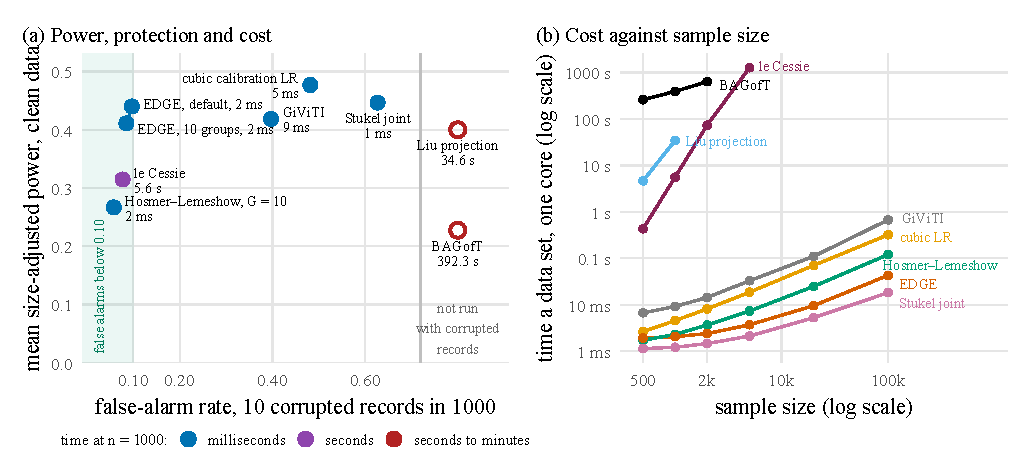
\includegraphics[width=\textwidth]{Fig15_cost}
\caption{Power, protection and cost of each test. (a)~Mean size-adjusted power on clean data over the
twenty scenarios on which all eight tests were run, against the false-alarm rate with ten corrupted
records in $1000$ (corruption C1); the shaded strip is below $0.10$, and each label gives the median
time for one data set at $n=1000$. The two resampling tests were not run with corrupted records.
(b)~Median time against sample size on one core, both axes logarithmic. EDGE is timed in the
implementation that forms no $G\times G$ matrix; each rival is timed as published. EDGE is shown at
the default partition and at ten groups; Online Resource~1, Section~S12, gives the timing protocol.}
\label{fig:cost}
\end{figure}

\section{Computation and implementation}\label{sec:computation}

Throughout this section $n$ is the number of records, $p$ the number of columns of the model matrix
$X$, intercept included, $G$ the number of groups and $d$ the number of basis columns. In the designs of
this paper $p$ and $d$ are small: $d$ is $1$ or $3$, or one more in the external mode.

\subsection{The algorithm and its cost}\label{sec:algorithm}

We take as given the fitted logistic model, that is, the fitted risks $\hat\pi_i$, the model
matrix $X$ and the fitted weights $W$. Every test of the fitted model needs this fit, and EDGE needs it
only once. Given the fit, EDGE is computed in seven steps.

\begin{enumerate}
\item \textbf{Sort and group.} Rank the records by fitted risk, ties in the order of the records, and
assign the record of rank $R_i$ to group $\lceil R_iG/n\rceil$. A stable sort costs $O(n\log n)$
operations. This is the only step whose cost grows faster than linearly in $n$.
\item \textbf{Group sums and grouped residuals.} In one pass over the records, accumulate for each
group the observed events $O_g$, the expected events $E_g$, the binomial variance $V_g$ and the count
of records, and from them $\pibar_g$ and the residual $r_g$ of \eqref{eq:resid}, at a cost of $O(n)$.
\item \textbf{Estimation adjustment.} In the same pass, accumulate the $G\times p$ matrix $U$ of
\eqref{eq:omega}, at a cost of $O(np)$. Form the information matrix $X^\top WX$, at a cost of $O(np^2)$,
and factor it, at a cost of $O(p^3)$. The $G\times G$ covariance $\Omega$ is not formed, because the
test needs only its products with the $d$ basis columns (step~6). In the external mode this step is
skipped, because $\Omega=I_G$.
\item \textbf{Basis.} Evaluate the $d$ shape functions of Section~\ref{sec:bases} at the $G$ group
means $\pibar_g$, and orthogonalise the columns of $Z$, at a cost of $O(Gd^2)$.
\item \textbf{Projection.} Compute $Z^\top r$, at a cost of $O(Gd)$, and the statistic $S$ of
\eqref{eq:stat} by solving a $d\times d$ system, at a cost of $O(d^3)$.
\item \textbf{Eigenvalues.} Compute the $d\times d$ matrix $(Z^\top Z)^{-1}Z^\top\Omega Z$ of
Theorem~\ref{thm:null} as $Z^\top\Omega Z=Z^\top Z-(Z^\top U)(X^\top WX)^{-1}(U^\top Z)$, which costs
$O(Gdp+dp^2+d^2p)$ and never forms $\Omega$, and its eigenvalues, at a cost of $O(d^3)$. Forming $\Omega$
first would cost $O(G^2(p+d))$ operations and $O(G^2)$ memory.
\item \textbf{Reference distribution.} Match the first two moments of the weighted sum in
\eqref{eq:wchi2} by a scaled chi-squared variable $c\,\chi^2_\nu$, with
$\nu=(\sum_j\lambda_j)^2/\sum_j\lambda_j^2$ and $c=\sum_j\lambda_j^2/\sum_j\lambda_j$, and report
$p=\Pr(\chi^2_\nu>S/c)$ \citep{satterthwaite1946}. This costs $O(d)$ operations and one evaluation of
the chi-squared distribution function.
\end{enumerate}

The total cost, given the fit, is therefore
\[
O\bigl(n\log n+np^2+p^3+Gd(d+p)+dp^2+d^3\bigr)=O\bigl(n\log n+np^2\bigr),
\]
because $G\le n$, $p\le n$ and $d$ is bounded. The sort dominates only when $p^2$ is small next to
$\log n$; otherwise forming the information matrix dominates, as it does in the fit itself. The memory
needed beyond the data is $O(Gp)$.

The avoided $G\times G$ term matters at the default partition, $G=\max(10,\lceil n/25\rceil)$, where it
grows with the square of $n$; at $n=100{,}000$ there are $4000$ groups. The timed implementation of
EDGE forms no $G\times G$ matrix and is in the reproducibility archive; the CRAN release of the package
forms $\Omega$. The two return identical results up to rounding: over $250$ data sets and $6600$ settings, covering
the three bases, both weightings, both partitions and both modes, the largest differences were
$9.3\times10^{-10}$ in the statistic and $1.4\times10^{-11}$ in the $p$-value. Forming $\Omega$ made
EDGE $1.6$ times slower at $n=500$ and $11$ times slower at $n=100{,}000$, where it took $0.47$ seconds
against $43$ milliseconds.

\subsection{A reference distribution without resampling or refitting}\label{sec:noresampling}

The weights of the reference distribution of Theorem~\ref{thm:null} are the eigenvalues of a $d\times
d$ matrix built from quantities that the fit has already produced. No second model fit, no bootstrap
sample and no random split is needed. Three consequences follow.

First, the test costs about as much as the other tests that need no resampling. Every timing was taken on one
core of an AMD Ryzen 9 3900X processor with $32$ gigabytes of memory, in R 4.4, with the linear-algebra
library held to one thread and nothing else running. At $n=1000$, EDGE takes $2$ milliseconds, Stukel's joint
score test $1$, the Hosmer--Lemeshow statistic $2$, the cubic calibration test $5$ and the GiViTI belt
$9$ (Figure~\ref{fig:cost}). At $n=100{,}000$ EDGE takes $43$ milliseconds, Stukel's score $18$ and the
Hosmer--Lemeshow statistic $120$. The Liu projection test draws $B=250$ bootstrap samples and takes
$35$ seconds at $n=1000$. BAGofT refits the model $(1+\textit{nsim})\times\textit{nsplits}$ times,
$10{,}100$ model fits at its defaults; it takes $392$ seconds at $n=1000$ and ten minutes at $n=2000$.
Le Cessie's smoothed test needs no resampling, but in its published form it multiplies $n\times n$
matrices, so its cost grows with the cube of $n$: $5.6$ seconds at $n=1000$, $74$ seconds at $n=2000$
and $21$ minutes at $n=5000$, where EDGE takes $4$ milliseconds. Its $n\times n$ kernel would need about
$10$ gigabytes on the $35{,}000$ patients of each half of the cohort of Section~\ref{sec:realdata}, so
it was not run there.

Second, the $p$-value is a deterministic function of the data. It carries no Monte Carlo error and
does not depend on a random seed, whereas the two resampling tests return $p$-values on grids of
$1/100$ and $1/250$.

Third, the test can be run wherever it is needed: on every replicate of every scenario of this paper,
where the three slow rivals were run only on subsets, and across partitions. Because its degrees of
freedom do not depend on $G$ (Theorem~\ref{thm:growingG}), a sweep over partitions costs one sort in
all and one pass for each partition (Section~\ref{sec:realpartition}).

\subsection{The external mode and the streaming form}\label{sec:streamcomp}

In the external mode $\Omega=I_G$ and a constant column is added to the basis
(Section~\ref{sec:null}). Step~3 of the algorithm disappears, and the model matrix is not needed. All
$d+1$ eigenvalues of step~6 equal one, so the Satterthwaite approximation of step~7 returns the
chi-squared distribution on $d+1$ degrees of freedom exactly. The cost is $O(n\log n+Gd^2)$. On one
core, the external mode at ten groups took about $0.3$ milliseconds at $n=1000$ and $12$ milliseconds at
$n=100{,}000$. The test of \citet{sadatsafavi2024nonparametric}, from the R package \texttt{cumulcalib},
took about $0.25$ and $14$ milliseconds on the same data sets.

The external mode can also be computed as a stream, which suits the monitoring of a deployed model.
The equal-frequency groups of step~1 are replaced by cut points $0<c_1<\dots<c_{G-1}<1$ fixed in
advance from reference predictions, without any outcome. The monitor holds four sums for each group:
the observed events $O_g$, the expected events $E_g$, the binomial variance $V_g$ and the count $m_g$.
These are all the statistic needs, because $r_g=(O_g-E_g)/\sqrt{V_g}$ and $\pibar_g=E_g/m_g$.

\begin{enumerate}
\item \textbf{Update.} When a patient with prediction $p_i$ and outcome $y_i$ arrives, find the
patient's group by a binary search among the $G-1$ cut points, at a cost of $O(\log G)$, and add $y_i$,
$p_i$, $p_i(1-p_i)$ and $1$ to the four sums of that group. No earlier record is kept or revisited.
\item \textbf{Test.} At any time, compute the residuals and the group means from the $G$ summaries,
evaluate the basis with its constant column over the non-empty groups, and compute $S_n=r^\top P_Zr$
through a QR decomposition of a $G\times k$ matrix, where $k$ is the rank of the basis ($d+1$ once
$d+1$ groups with distinct mean risks are non-empty), at a cost of $O(Gk^2)$.
\end{enumerate}

The memory needed is $O(G)$, whatever the length of the stream. Each of the four sums is a sum of terms
that depend on one patient alone, so the streamed statistic is the same for every order and every
division into batches, and equals the external-mode statistic computed in one pass with the same cut
points. Under a calibrated model the statistic has a chi-squared reference on $k$ degrees of freedom
asymptotically, as every non-empty group grows, however unequal the groups become (Online Resource~1,
Section~S8, proves these three properties). The price of fixed cut points is that the groups drift
away from equal size when the risk mix of the monitored patients changes, and small groups give weaker
protection against corrupted records (Proposition~\ref{prop:bounded}). On one core, after a million
patients had been added, adding a hundred more took about half a millisecond and computing the test
about $1.5$ milliseconds.

In a simulation of the streaming form fixed before it was run, at ten groups and with $2000$
replicates, the level was $0.047$ and $0.054$ after $10{,}000$ and $100{,}000$ patients, and $0.050$ and
$0.052$ when every monitored patient came from a risk distribution different from the reference. The
test detected an overfitted model, calibration slope $0.8$, in $0.99$ of replicates after $2000$
patients (Online Resource~1, Section~S8). The statistic accumulates since deployment; to follow drift,
the summaries are restarted each period and each period is tested on its own. One test at any time is
valid, but acting on the first rejection over repeated looks is not: ten looks at $5\%$ raised the
false-alarm rate to $0.21$, and splitting the level over ten looks fixed in advance, $0.5\%$ each,
brought it to $0.030$.

\subsection{Software}\label{sec:software}

The test and its comparators are implemented in the R package \texttt{ebrahim.gof}
\citep{ebrahim2025gof}, available from CRAN (Section~\ref{sec:algorithm} compares its timing with the
implementation timed here).

\begin{itemize}
\item \texttt{edge.gof(fit)} runs EDGE on a fitted binomial \texttt{glm} and reports the verdict at the
default partition and, as a robustness check, at ten groups; the degrees of freedom reported are the
effective $\nu$ of step~7. The argument \texttt{G = 10} gives the ten-group partition, \texttt{basis =
"sym"} or \texttt{"stukel"} the other bases, and \texttt{weights = "score"} the score form.
\item \texttt{edge.gof(y, predicted\_probs = p, external = TRUE, G = 10)} runs the external mode on
outcomes \texttt{y} and frozen predictions \texttt{p}; with \texttt{G} set accordingly it reproduces
every statistic of Section~\ref{sec:realdata}.
\item \texttt{run.all.gof()} fits the model once and returns every comparator of
Section~\ref{sec:comparators} except the cubic calibration test.
\item \texttt{run.all.external(y, p)} runs the external mode beside the other external-validation
tests, Cox's recalibration test and the calibration intercept and slope among them.
\item \texttt{edge.stream()} creates the monitor of Section~\ref{sec:streamcomp}; \texttt{update()} adds
a batch of outcomes and predictions and \texttt{summary()} returns the test at any time.
\end{itemize}

\section{Corrupted records}\label{sec:contamination}

\subsection{False alarms from a handful of records}\label{sec:c1}

Table~S5 of Online Resource~1 gives the false-alarm rate of every test under corruption C1. The model
under test is effectively the clean one: over the $24$ scenarios of C1 the slope on the corrupted
covariate moves by less than $5\%$, the slope on the second covariate by at most $1.9\%$ and the
intercept by at most $0.02$ on the linear-predictor scale. The mean absolute distance of the clean
records' fitted risks from the true risk, an integrated calibration index \citep{austin2019ici}, is
$0.0185$ with one exaggerated record in $1000$ and $0.0199$ with ten, against $0.0189$ without
corruption. A test that rejects here is reacting to a few records, not to the model that is used for
everyone else.

One corrupted record in a thousand moves every record-level test. Stukel's joint score rises from the
nominal level to $0.121$, its one-parameter form to $0.115$, the cubic calibration test to $0.127$ and
the GiViTI belt to $0.089$. EDGE reads $0.056$ with the cubic basis and $0.058$ with the
symmetric basis. At five corrupted records the record-level tests are between $0.25$ and $0.40$ and
EDGE is still at $0.057$. At ten, Stukel's joint score reaches $0.627$, rejecting a correct
model more often than not, while EDGE reads $0.097$. Every test holds its level in the same design
without corruption, so the difference is not that one test is conservative.

The pooled tests are protected, as Section~\ref{sec:mechanism} predicts. Le Cessie's smoothed test
reads $0.055$, $0.052$, $0.052$ and $0.077$ at one, two, five and ten corrupted records. The
Hosmer--Lemeshow statistic and the Pigeon--Heyse test at ten groups, under the exaggeration, stay at
or below $0.058$ up to ten
corrupted records in $1000$ and twenty-five in $5000$ (Table~\ref{tab:severity}), although the
Pigeon--Heyse test is conservative throughout. Grouped tests with small extreme groups are not
protected: the equal-width Hosmer--Lemeshow statistic reaches $0.592$ at ten corrupted records in
$1000$, and the two tests that group on the covariates reach $0.542$ (Tsiatis) and $0.606$ (Xie). In a
smaller study of three corrupted records in $500$ with the covariate multiplied by four or by eight,
$100$ replicates a scenario, BAGofT and EDGE with the cubic basis gave no sign of moving, while the
projection test reached $0.22$ at $\times8$ and EDGE with the symmetric basis $0.20$; with $100$
replicates a rise of a few points could not be seen (Online Resource~1, Section~S3).

Wrong outcomes are a different matter. When the ten highest-risk records in a thousand have their
event erased (C2), every test rejects more often, EDGE included, at $0.667$ against Stukel's $0.718$ and
the cubic test's $0.837$; a calibration test should find missing events. A unit error that makes
predictions milder (C3) moves no test under the logistic truth, and duplicated records (C4) leave every
test between $0.040$ and $0.071$ (Online Resource~1, Section~S2).

\subsection{What protects: pooling with unit weights}\label{sec:whatprotects}

A direction that is bounded, a polynomial in the predicted risk rather than in the logit, might
protect without grouping. On the same data sets (Online Resource~1, Section~S10) it does not. With one
exaggerated record in $1000$ the ungrouped score test for EDGE's cubic directions, which we call the
ungrouped twin, rejects a correct model in $0.166$ of replicates and with ten in $0.641$, against
$0.047$ and $0.101$ for EDGE at the default partition and $0.051$ and $0.066$ at ten groups. EDGE with
one record a group behaves like Stukel's test ($0.148$ and $0.594$). Spiegelhalter's $z$, whose normal
reference ignores the fit, rejects in $0.118$ and $0.546$ when read at the critical value of its own
uncorrupted null. Grouping alone is not enough either: EDGE's score form, which uses the same groups
but divides by the information its directions keep after the fit, rejects in $0.087$ and $0.463$ at ten
groups, against $0.056$ and $0.085$ for the unit form. The weighted grouped tests of
\citet{hosmer2002goodness}, which weight each record within its group by a function of its covariates,
reach $0.18$ and $0.27$ with ten exaggerated records and $0.68$ and $0.82$ with ten reversed ones.

On frozen predictions, where nothing is refitted, the ungrouped twin reads $0.061$ and $0.096$ with one
and ten exaggerated records, but still $0.311$ with ten reversed records, where EDGE at ten groups reads
$0.082$. Two things therefore make a test fragile: the refit, whose effect a score test magnifies by
dividing by the information left after it, and directions that lean on the few most extreme records.
EDGE's unit form avoids both, because its divisor is the variance of the clean groupmates. The same
holds with twelve covariates at $n=2000$: with ten reversed records EDGE reads $0.091$ at the default
partition and $0.048$ at ten groups, against $0.315$ for Stukel's test and $0.292$ for the ungrouped
twin. Influence diagnostics are no remedy. Removing every record whose $\Delta X^2$ exceeds $4$ or
whose $\Delta\beta$ exceeds $1$ \citep{pregibon1981logistic,hosmer2013applied} made every test reject a
correct model in more than $0.95$ of replicates. The milder rule, $\Delta\beta>1$ alone, removed no
record, because at an extreme prediction a corrupted record's leverage and residual are both small on
the fitted scale.

\subsection{The partition, not the contamination rate}\label{sec:partition}

A second study varied the number of groups with the data held fixed (Figure~\ref{fig:partition}). The
contamination \emph{rate} does not decide the outcome: twenty-five corrupted records in $5000$ and five
in $1000$ are both $0.5\%$, and EDGE reads $0.152$ and $0.048$. The partition does: at $n=5000$ with
twenty-five corrupted records the same data give $0.062$ at ten groups and $0.152$ at two hundred; with
fifty they give $0.094$ and $0.726$. Without corruption the rate stays between $0.046$ and $0.057$ at
every partition.

\begin{figure}[htbp]\centering
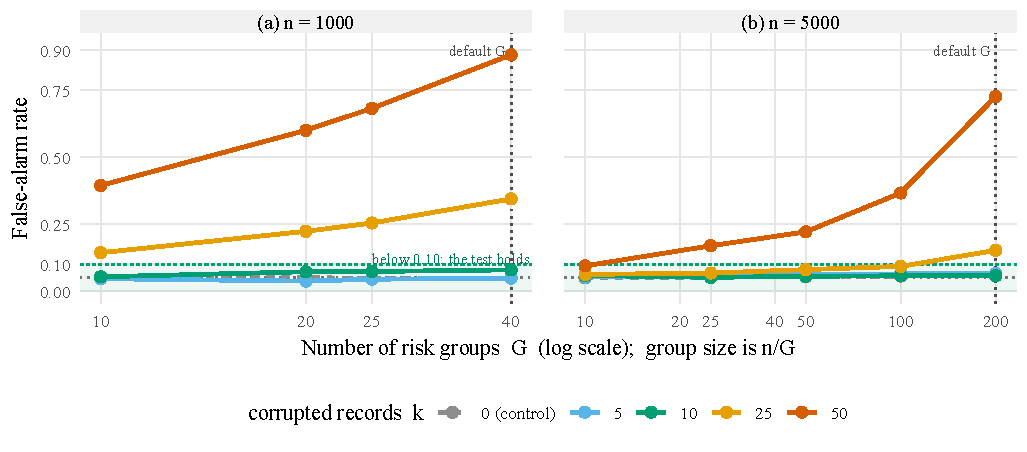
\includegraphics[width=\textwidth]{Fig12_partition}
\caption{False-alarm rate of EDGE (cubic basis, unit form) under a correct model with $k$ corrupted
records, against the number of risk groups; (a)~$n=1000$, (b)~$n=5000$. The shaded area lies below
$0.10$, the dotted line marks the default partition and the dashed grey line is the uncorrupted
control.}
\label{fig:partition}
\end{figure}

The reason is in \eqref{eq:twomoments}. Corrupted covariates produce the most extreme predictions, so
they fill the top and bottom groups first. At the default partition the group size $m$ stays near
twenty-five, so the \emph{count} of corrupted records decides: ten in $1000$ put an average of $3.7$
into the top group and the test reads $0.079$, and fifty in $5000$ put $17.8$ there, leaving about seven
clean members, and it reads $0.726$. At ten groups $m=n/10$ grows with the sample; the same data put
$4.0$ and $19.9$ records into top groups of $100$ and $500$, and the test reads $0.053$ and $0.094$.
(The partition study drew its own data sets, so its rates differ from those of
Table~\ref{tab:severity} by Monte Carlo error.)

\subsection{The severity of the error}\label{sec:severity}

A sign error (C1$'$) reverses the prediction instead of exaggerating it, $\theta$ in
\eqref{eq:twomoments} rises from about $0.3$ to about $0.7$, and the fit moves more, by $14\%$ in the
slope; the two channels were not separated. Table~\ref{tab:severity} gives both errors. With the cubic basis at the default partition EDGE
holds to about two corrupted records in $1000$ and five in $5000$ under the sign error, against about
ten under the exaggeration: at ten records in $1000$ it reads $0.381$. The symmetric basis at the
default partition holds to ten in both sample sizes, reading $0.098$ and $0.058$, although against many
exaggerated records it is no better than the cubic basis ($0.745$ at fifty in $5000$). At ten groups,
under the sign error, the symmetric basis is less protected than at the default partition ($0.431$
against $0.098$ at ten records in $1000$), which we observe but cannot explain from
\eqref{eq:twomoments}. Whatever the setting, the ordering of the tests is unchanged: at one reversed
record in a thousand EDGE reads $0.054$ against Stukel's $0.364$, the cubic test's $0.389$ and the belt's
$0.268$.

\input{tab_severity}

\subsection{Protection when records may be wrong}\label{sec:edgefr}

For the cubic basis the partition sets a trade-off between power and protection. The default
partition has more power: on clean data it leads ten groups by $0.017$ on average over the $158$
scenarios, and by much more when the misfit is confined to the extreme risks. With the true risk of the
top $2\%$ of patients $40\%$ below its prediction its size-adjusted power is $0.42$ at $n=1000$, against
$0.19$ at ten groups (Online Resource~1, Section~S10). Ten groups tolerate more corrupted records: they
read $0.085$ with ten exaggerated records in $1000$ and $0.107$ with fifty in $5000$, where the default
partition reads $0.097$ and $0.740$, and under the sign error $0.081$ with five records in $1000$ and
$0.077$ with ten in $5000$. The partition is therefore chosen in the analysis plan, before the results
are seen: running both and reporting the more convenient would bring back the dependence on $G$ that
Section~\ref{sec:realpartition} shows for the Hosmer--Lemeshow test. Pooling only the two extreme groups
matched ten groups up to about ten corrupted records in $1000$, with the same power, and was less
protected beyond (Online Resource~1, Section~S5).

At ten groups the plain Hosmer--Lemeshow statistic holds its level further than EDGE once there are
more than a few reversed records: $0.099$ against $0.182$ at ten in $1000$, and $0.126$ against $0.249$ at
twenty-five in $5000$. What EDGE offers at ten groups is power, $0.411$ against $0.267$
(Section~\ref{sec:census}).

\subsection{The cost in power, and robust alternatives}\label{sec:cost}\label{sec:robustest}

The protection costs power when a real misfit and corrupted records occupy the same extreme groups.
Read at the critical value of its own contaminated null, which the analyst cannot know but which
isolates the misfit, EDGE against a
complementary log--log truth at $n=1000$ falls from $0.826$ on clean data to $0.771$ at one corrupted
record and $0.648$ at ten; against a probit truth at $n=5000$ it falls from $0.278$ to $0.233$ at five
and $0.207$ at ten. Beyond the protected range the test has no power left: at twenty-five corrupted
records in $5000$, read at its contaminated null, it is $0.045$ against the probit truth (Online
Resource~1, Section~S14).

A robust fit is no substitute. After the Huber-type quasi-likelihood fit of
\citet{cantoni2001robust}, which puts no weight on the covariates, five of ten tests no longer hold
their level on clean data, and none of the other five has its false alarms reduced; at ten corrupted
records EDGE reads $0.089$ after maximum likelihood and $0.087$ after the robust fit (Online
Resource~1, Section~S4). Robust fits that also down-weight outlying covariates exist
\citep{bianco1996robust,croux2003implementing}; the Bianco--Yohai fit was specified for this study but
was not run.

A robust \emph{test} protects less than pooling. The robust quasi-deviance test of
\citet{cantoni2001robust} for Stukel's two constructed covariates, in its Mallows form, which also
down-weights records of high leverage, holds below $0.10$ with one or two corrupted records. With ten
exaggerated records it reads $0.168$ and with ten reversed ones $0.789$, where EDGE at ten groups reads
$0.063$ and $0.192$, and its power against a complementary log--log truth is $0.610$, against EDGE's
$0.779$ (Online Resource~1, Section~S14).

\section{A clinical cohort and external validation}\label{sec:realdata}

The Diabetes 130-US hospitals cohort \citep{strack2014impact,clore2014uci} records $101{,}766$
admissions of patients with diabetes at $130$ hospitals over ten years, with readmission within
thirty days as the outcome. Following the data set's authors we keep one admission per patient, the
first, excluding admissions that ended in death or discharge to hospice and the three records whose sex
is unknown. That leaves $69{,}987$ patients. We split them in half at random, fitted a logistic model on
the first half, and froze its predictions for the second. The model uses the routinely recorded
predictors: age, sex, length of stay, the numbers of laboratory procedures, other procedures,
medications, outpatient, emergency and inpatient visits in the preceding year and diagnoses, insulin
use in four levels, a change of diabetes medication, and any diabetes medication. No attempt was made
to make the model fit well or badly; it has an area under the curve of $0.60$ on the validation half.

\subsection{The partition on real data}\label{sec:realpartition}

On the development half ($34{,}993$ patients) the fit is checked as the partition is refined from
$G=10$ to $G=2000$ (Figure~\ref{fig:diabetes}(b)). EDGE rejects at every partition,
with $p$ between $4\times10^{-5}$ and $7\times10^{-4}$. The Hosmer--Lemeshow statistic rejects at ten
groups ($p=0.041$) and at no finer partition, with $p$ between $0.10$ and $0.50$ from twenty groups on;
its Farrington correction behaves the same way. Two analysts who chose $G=10$ and $G=50$ would reach
opposite conclusions about the same model \citep{paul2013power}; EDGE's reference does not change
with the number of groups (Theorem~\ref{thm:growingG}).

\subsection{Validation}\label{sec:realvalidation}

On the validation half ($34{,}994$ patients) nothing is refitted, so EDGE is in the external mode, with
the intercept as a fourth column. The calibration intercept-and-slope test of \citet{cox1958} and
\citet{Miller1991} rejects: the calibration slope is $0.85$, and the likelihood-ratio statistic is
$13.3$ on two degrees of freedom, $p=0.001$. The miscalibration is small in absolute terms (integrated
calibration index $0.007$; \citealp{austin2019ici}); with $35{,}000$ patients the tests detect it, and
whether it matters clinically is a separate question \citep{nattino2020assessing,vancalster2019}.
EDGE rejects at every partition, with $S$ between $23$ and $41$ on four degrees of freedom and $p$
between $1\times10^{-4}$ and $3\times10^{-8}$, and the GiViTI belt in its external mode rejects as well
($p=1.5\times10^{-8}$). The Hosmer--Lemeshow statistic rejects at five of the eight partitions.

The shape of the miscalibration is not a simple tilt. Figure~\ref{fig:diabetes}(a) shows the top decile
and the second over-predicted and the middle deciles under-predicted, by $1.0$ to $1.5$ percentage
points in deciles three, five, six and nine. A
grouped test restricted to the intercept and slope columns does not reject at any partition ($p$
between $0.08$ and $0.34$): at ten groups only about $2$ of the statistic's $23$ lie in those
directions, and the rest in the curvature. The grouped tilt is less sensitive than the record-level
Cox--Miller test to this slope, so EDGE complements the calibration intercept and slope and does not
replace them. Online Resource~1, Section~S15, draws the grouped residuals with the
projection whose squared length is the statistic.

\begin{figure}[htbp]\centering
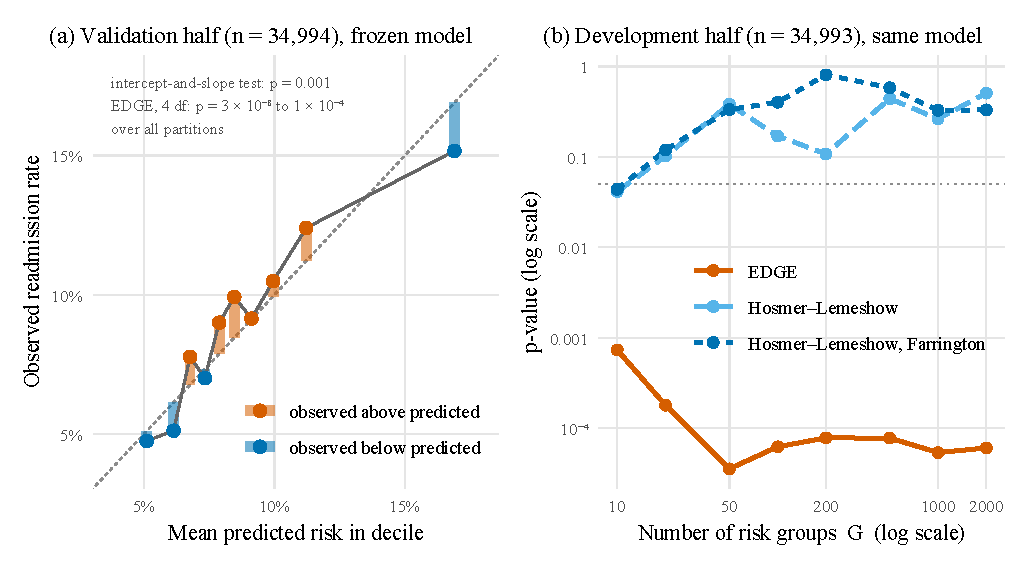
\includegraphics[width=\textwidth]{Fig10_diabetes}
\caption{The Diabetes-130 cohort. (a)~Validation half, frozen model: observed readmission rate against
mean predicted risk in ten equal-frequency risk groups. (b)~Development half: the $p$-value of EDGE,
the Hosmer--Lemeshow statistic and its Farrington correction as the partition is refined from $G=10$ to
$G=2000$; the dotted line is $0.05$.}
\label{fig:diabetes}
\end{figure}

\subsection{Corrupted records in this cohort}\label{sec:realcorrupt}

On the real covariates and the frozen predictions of the validation half we draw the outcome from the
model itself, so that the model is correct by construction and every rejection is a false alarm. Then
$k$ records have one covariate multiplied by four, with their prediction recomputed at the corrupted
value and their outcome kept; $500$ replicates at each $k$. Corrupting the number of laboratory
procedures, which has a small coefficient, moves no test at any $k$. The number of previous inpatient
admissions has the model's largest coefficient, $0.38$, but only $12\%$ of patients have any previous
admission, so of a hundred corrupted records about twelve change. Four previous admissions is a
plausible value, so this error passes a range check. It is the covariate on which the experiment could
show most, and it was chosen for that reason, by a rule fixed before it was run, after the first showed
nothing (Table~\ref{tab:cohortcorrupt}).

\begin{table}[htbp]\centering\small
\caption{False-alarm rate on the cohort's validation half ($n=34{,}994$) when $k$ records have the
number of previous inpatient admissions multiplied by four and the model is otherwise correct by
construction. The grouped tests are in the external mode; the default partition has $1400$ groups.
$500$ replicates at each $k$.}
\label{tab:cohortcorrupt}
\begin{tabular}{rrrrrr}\hline
$k$ & EDGE (default $G$) & EDGE ($G{=}10$) & HL ($G{=}10$) & Stukel joint & cubic LR \\ \hline
0   & 0.050 & 0.044 & 0.048 & 0.050 & 0.042 \\
10  & 0.042 & 0.042 & 0.050 & 0.102 & 0.080 \\
50  & 0.086 & 0.060 & 0.060 & 0.254 & 0.198 \\
100 & 0.080 & 0.054 & 0.048 & 0.448 & 0.314 \\ \hline
\end{tabular}
\end{table}

About twelve changed records among $34{,}994$ patients raise Stukel's score test to $0.448$ and the
cubic calibration test to $0.314$. EDGE stays below $0.09$ at the default partition and within Monte
Carlo error of the nominal level at ten groups.

\subsection{External validation in simulation}\label{sec:extval}

A simulation of external validation in one design with five covariates (Online Resource~1, Section~S7)
sets EDGE against the usual tests there. At ten groups its mean size-adjusted power over ten
departures is $0.415$, against $0.420$ for the GiViTI belt and $0.410$ for Cox's recalibration test,
which in most data sets return the same $p$-value. On a shift and a threshold term Cox's test leads by
up to $0.14$ and the belt by up to $0.15$; EDGE leads by up to $0.21$ on a U-shaped term and an
interaction. With ten reversed
records in $1000$ EDGE reads $0.082$, below the bar of $0.10$, where Cox's test reads $0.158$ and the belt
$0.347$; the Hosmer--Lemeshow statistic and Spiegelhalter's $z$ stay below it too, with less power
($0.335$ and $0.271$).

The cumulative-sum test of \citet{sadatsafavi2024nonparametric} was added to this study on the same
data sets, under its own specification fixed before it ran. It held its level, at $0.046$ to $0.048$,
and its mean size-adjusted power was $0.380$: EDGE at ten groups was ahead by $0.035$ (Monte Carlo
$95\%$ interval $0.028$ to $0.042$), and Cox's test by $0.030$ ($0.024$ to $0.035$). The cumulative-sum
test led EDGE by $0.066$ on the shifts and by $0.066$ on the threshold terms; EDGE led it by $0.023$ on
the slopes, $0.118$ on the U-shaped terms and $0.167$ on the interactions. Under corrupted records the
cumulative-sum test stayed below $0.10$ in all eight settings, between $0.035$ and $0.055$, and with ten
reversed records it read $0.052$, against $0.082$ for EDGE. Protection against corrupted covariates is
therefore not unique to EDGE in external validation: the cumulative-sum test has it too, and slightly
more against sign errors. What EDGE adds there is power against U-shaped and interaction departures.
Section~\ref{sec:streamcomp} gives the streaming form of the external mode and its simulated level.

\section{Discussion}\label{sec:discuss}

\subsection{What grouping still buys}\label{sec:asymmetry}

Grouping was introduced so that a goodness-of-fit test for logistic regression would have a reference
distribution. It also bounds the influence of a record whose prediction is wrong
(Section~\ref{sec:mechanism}). On clean data EDGE is comparable to Stukel's score test and the cubic
calibration test. Its advantage is that it keeps its level when a few records are wrong, at a modest
cost in power, most when the misfit lies in the extreme risk groups (Sections~\ref{sec:edgefr}
and~\ref{sec:cost}).

The protection does not extend to wrong outcomes, which a calibration test should detect. A grouped
test that rejects while covariate errors are suspected is therefore reporting something other than
those errors; the same test rejecting while outcome errors are suspected may be reporting them, and the
data should be checked before the model is rebuilt. Tolerating a few wrong inputs is the right
behaviour when the question is whether the model is right, at development and validation. Once the
model is deployed, finding a patient whose input is wrong is the job of checks at data entry, not of a
calibration test.

\subsection{Recommended use}\label{sec:whentouse}

\begin{enumerate}
\item Use the cubic basis in its unit form at the default partition, $G=\max(10,\lceil n/25\rceil)$, and
      report the calibration intercept and slope beside it; \texttt{edge.gof(fit)} reports it beside
      ten groups.
\item If the data are known to carry entry errors in the predictors, as routinely collected records
      may, plan ten groups instead, \texttt{edge.gof(fit, G = 10)}: they tolerate about ten exaggerated
      or five reversed records in $1000$, at a cost of $0.017$ in mean power and about half the power
      against misfit confined to the extreme risks. Decide this before seeing the results. If only the
      default partition rejects, check the records in the extreme groups. If the suspected errors are
      reversals only, up to about ten in $1000$, the symmetric basis at the default partition holds
      further. We had expected the default partition to hold over $0.1\%$ to $0.5\%$ contamination; at
      the upper end it does not (Section~\ref{sec:partition}). If protection
      matters more than power, use the Hosmer--Lemeshow statistic at ten groups. Beyond a few tens of
      corrupted records, clean the data; influence diagnostics do not find them.
\item When the departure feared is a symmetric change in both tails, use the symmetric basis; on clean
      data with high discrimination or a strongly skewed covariate, in its score form,
      \texttt{edge.gof(fit, basis = "sym", weights = "score")}.
\item When a frozen model, logistic or not, is validated on new patients, use the external mode at ten
      groups, in which Proposition~\ref{prop:bounded} holds exactly because nothing is refitted:
      \texttt{run.all.external(y, p)} reports it beside Cox's recalibration test and the calibration
      intercept and slope. When the departure feared is a shift in the overall risk or a threshold
      effect, use the test of \citet{sadatsafavi2024nonparametric} beside EDGE or instead of it.
\item The study covers six departure families with one to three covariates (five in external
      validation, twelve in one design), one real cohort, and covariate errors that multiply a value by
      four or minus four, with three other mechanisms beside them; errors correlated with the outcome
      were not examined. Robust tests were compared in the form of Stukel's test at $n=1000$, the
      weighted grouped tests of \citet{hosmer2002goodness} with their general-purpose weight, and the
      test of \citet{sadatsafavi2024nonparametric} only on frozen predictions, in one design. Results
      outside these settings should be checked by simulation, for which the archive gives the code.
\end{enumerate}

\subsection{When another test is better}\label{sec:whennot}

Table~\ref{tab:whennot} lists the settings in which the study found a better choice; for each, the
best of EDGE's forms is compared with the rival named.

\begin{table}[htbp]\centering
\caption{Settings in which another test, or another form of EDGE, is the better choice.
Power comparisons are on clean data; every false-alarm rate quoted, and the last two rows, are under
corrupted records.}
\label{tab:whennot}
\small
\begin{tabular}{>{\raggedright\arraybackslash}p{0.26\textwidth}>{\raggedright\arraybackslash}p{0.21\textwidth}>{\raggedright\arraybackslash}p{0.43\textwidth}}\toprule
Setting & Better choice & Evidence \\ \midrule
Scarce events ($12\%$), clean data & GiViTI belt & The belt leads EDGE by up to $0.152$;
but it reads $0.089$ false alarms at one corrupted record in $1000$ and $0.397$ at ten. \\
A single smooth bend, clean data & Cubic calibration test or GiViTI belt & The cubic test leads in $15$
of $21$ asymmetric-link scenarios (mean $0.741$, belt $0.744$, EDGE $0.669$; largest gap $0.208$); but it
reads $0.127$
and $0.482$ false alarms at one and ten corrupted records in $1000$, where EDGE reads $0.056$ and
$0.097$. \\
A curve that crosses the diagonal twice & BAGofT or le Cessie's test & BAGofT rejects $155$ of $200$
replicates, EDGE $18$. \\
Rough or oscillating misfit & BAGofT & $1.000$ and $0.805$ on the fastest oscillation and the sawtooth,
against $0.438$ and $0.093$ for the best form of EDGE, the Stukel basis. \\
Frozen model, a shift or a covariate threshold & Test of Sadatsafavi and Petkau & It leads EDGE at ten
groups by $0.066$ on both families in external validation, and stays below $0.10$ false alarms in all
eight corrupted settings ($0.052$ with ten reversed records in $1000$). \\
An omitted interaction & Le Cessie's test & Leads in $11$ of $15$ binary and $8$ of $12$ continuous
interaction scenarios. \\
Symmetric tails, or a strongly skewed covariate & Symmetric basis, score form & Stukel's one-parameter
score leads the default basis by $0.062$ on symmetric tails and the unit symmetric form by $0.252$ under
a skewed covariate; the score form ties it on both ($-0.002$ on average over $32$ scenarios, $-0.007$
to $+0.012$ over the four skewed ones, where its level is $0.049$ to $0.057$). \\
Many reversed records, protection first & Hosmer--Lemeshow at ten groups & $0.099$ against $0.182$ for
EDGE at ten groups with ten reversed records in $1000$, and $0.126$ against $0.249$ with
twenty-five in $5000$; its power is lower. \\
Tens of corrupted records & Clean the data & At fifty in $5000$ the default reads $0.740$ and ten groups
$0.107$; at a hundred no setting holds, and a robust fit does not help. \\
\bottomrule
\end{tabular}
\end{table}

\subsection{Further work}\label{sec:limits}

In the development data the estimation adjustment $\Omega$ is derived here for logistic regression
only; its form for other models is left for further work. A quantity that predicts the whole partition
surface of Figure~\ref{fig:partition} is still missing. Since wrong predictions and wrong outcomes move
grouped and ungrouped tests differently, reading the two together may tell which kind of error is
present. A sequential reference that uses the dependence between looks, rather than spending the level
over them, would make the streaming form a true monitor.


\begin{appendices}
\appendix

\section{Assumptions and proofs}\label{app:proofs}

The proofs of Theorems~\ref{thm:null} and~\ref{thm:growingG} and of Proposition~\ref{prop:bounded} are
in Online Resource~1, Section~S11. This appendix states the assumptions, gives the limit of
Theorem~\ref{thm:growingG}, and outlines the arguments.

\paragraph{Assumptions} Theorem~\ref{thm:null} uses (A1)--(A4) and Theorem~\ref{thm:growingG} uses
(A2), (A3) and (A4$'$). \textbf{(A1)} The number of groups $G$ is fixed and equal-frequency grouping
gives $n_g/n\to1/G$ for every $g$. \textbf{(A2)} The covariates are independent and identically
distributed with $\mathbb{E}\|x\|^2<\infty$ and $n^{-1}X^\top WX\to J_0$ positive definite, so that
the maximum-likelihood expansion $\hat\beta-\beta=(X^\top WX)^{-1}X^\top(y-\pi)+o_p(n^{-1/2})$
holds. \textbf{(A3)} The true probabilities satisfy $\varepsilon\le\pi_i\le1-\varepsilon$ for a fixed
$\varepsilon>0$, so that $V_g/n_g$ is bounded away from zero. \textbf{(A4)} The distribution of the
linear predictor is continuous with positive density at its $G-1$ population quantiles, so that the
sample group boundaries converge to fixed population boundaries and the grouping map may be treated
as fixed, by the random-cell argument of \citet{Moore1975}. \textbf{(A4$'$)} For every $b$ in a neighbourhood of $\beta$ the distribution of $x^\top b$ is
absolutely continuous with density bounded above uniformly in $b$, and at $b=\beta$ the density of
$\eta$ is continuous and bounded away from zero on its support, which (A3) makes compact. Then
$F_\eta$ is a $C^1$ bijection of that support onto $[0,1]$, $q=F_\eta(\eta)$ is uniform, and the
quantile functions $Q_\eta$ and $Q_\pi=\mathrm{expit}\circ Q_\eta$ are $C^1$ with bounded
derivative. At fixed $G$, (A4$'$) implies (A4). Assumption (A3) restricts the asymptotic regime and
not the method; the size study of Section~\ref{sec:size} covers designs outside it.

\paragraph{The limit of Theorem~\ref{thm:growingG}} Let $\varphi=(\varphi_1,\dots,\varphi_d)^\top$ be
the shape functions of the theorem, $v(q)$ the value of $\pi(1-\pi)$ at quantile position $q$ and
$\kappa(q)=\sqrt{v(q)}\,\mathbb{E}[x\mid q]$. Then
\begin{equation}\label{eq:growingG}
S\rightsquigarrow\sum_{j=1}^d\lambda_j\chi^2_{1,j},\qquad \{\lambda_j\}=\text{eigenvalues of }
M^{-1}\Sigma,\quad \Sigma=M-KJ_0^{-1}K^\top,
\end{equation}
with $M=\int_0^1\varphi\varphi^\top dq$ and $K=\int_0^1\varphi\,\kappa^\top dq$, which do not depend
on $G_n$.

\paragraph{Outline of the proofs} For Theorem~\ref{thm:null}, a one-term expansion of $\hat\pi$ writes
$r$ as the grouped residual before fitting minus $U(X^\top WX)^{-1}$ times the score; a joint central
limit theorem gives $r\rightsquigarrow N(0,\Omega)$, and the quadratic form $r^\top P_Zr$ then has the
weights of \eqref{eq:wchi2}, which lie in $[0,1]$ because $0\preceq\Omega\preceq I_G$. For
Theorem~\ref{thm:growingG}, the statistic is written as a smooth-weighted sum of all $n$ residuals; a
central limit theorem is applied with population weights, the weights of the statistic are shown to be
uniformly close to those, which is where the rate condition $G_n/\sqrt{\log n}\to\infty$ enters, and
the fitting correction gives $\Sigma$ through a law of large numbers over the whole sample, not within a
group. For Proposition~\ref{prop:bounded}, the corrupted record enters its group only through $E_g$ and
$V_g$, which it changes by less than one and by at most $1/4$, whatever $\eta^{*}$; the ungrouped score
grows as $\eta^{*2}$ while the record's information vanishes.

\end{appendices}

\backmatter

\bmhead{Supplementary information}
Online Resource~1 holds the proofs, the pre-specified comparisons and the full results.

\bmhead{Acknowledgements}
All praise and thanks are due to Allah, by whose grace this work was completed.

\section*{Statements and Declarations}

\noindent\textbf{Funding.} No funding was received for conducting this study.

\smallskip\noindent\textbf{Competing interests.} The authors have no competing interests to declare
that are relevant to the content of this article. The R package \texttt{ebrahim.gof}, which
implements the test proposed here and several of its comparators, is written and maintained by the
first author and is distributed free of charge under the GPL-3 licence.

\smallskip\noindent\textbf{Ethics approval.} Not applicable. The work reports a simulation study and
an analysis of the Diabetes 130-US Hospitals data \citep{clore2014uci}, a de-identified public data
set released for secondary research; no individual patient was contacted and no identifiable data
were used.

\smallskip\noindent\textbf{Data availability.} No new patient data were generated. The clinical data
analysed in Section~\ref{sec:realdata} are publicly available from the UCI Machine Learning Repository
\citep{clore2014uci} and are described by \citet{strack2014impact}. The study specifications with the
SHA-256 hashes that fixed them before any result was computed, the per-replicate $p$-values of every
scenario and the scripts that build every table and figure are deposited in a public archive
\citep{edge2_repro_2026}.

\smallskip\noindent\textbf{Code availability.} The tests are implemented in the R package
\texttt{ebrahim.gof} \citep{ebrahim2025gof}, available from CRAN, where a single call to
\texttt{run.all.gof()} runs the whole battery and \texttt{run.all.external()} does the same for frozen
predictions. The simulation code is in the archive above.

\smallskip\noindent\textbf{Use of AI tools.} The authors used a large-language-model assistant
(Claude, Anthropic) to help write code for the simulations, analyses and software and to draft and
edit the wording and \LaTeX{} of the text. The authors designed the study, checked every result
against the deposited scripts and data, reviewed all code and text, and take full responsibility for
the content.

\smallskip\noindent\textbf{Author contributions.} E.K.E.: conceptualisation, methodology, formal
analysis, software, investigation, data curation, visualisation, writing (original draft). O.A.H.:
supervision, validation, writing (review and editing). A.E.: supervision, project administration,
validation, writing (review and editing). All authors read and approved the final manuscript.

\bibliography{refs}

\end{document}
